\documentclass[12pt]{article}

\usepackage[right=20mm, left=20mm]{geometry}
\usepackage{type1cm}
\usepackage{amssymb}
\usepackage[fleqn]{amsmath}
\usepackage{tikz}
\usepackage{multicol}
\usepackage{makecell}
\setlength{\columnsep}{1pt}
\usepackage{pgfplots}
\usepackage{float}
\usepackage{caption}
\usepackage{graphicx}

\usepackage{indentfirst}
\usepackage{lastpage}  
\usepackage{fancyhdr}
\pagestyle{fancy}

\usepackage[unicode=true,pdfusetitle,
 bookmarks=true,bookmarksnumbered=false,bookmarksopen=false,
 breaklinks=false,pdfborder={0 0 1},backref=false,colorlinks=false]
 {hyperref}

\makeatletter
\newenvironment{myalign*}{\ifvmode\else\hfil\null\linebreak\fi
  \hspace*{-\leftmargin}\minipage\textwidth
  \setlength{\abovedisplayskip}{0pt}%
  \setlength{\abovedisplayshortskip}{\abovedisplayskip}%
  \start@align\@ne\st@rredtrue\m@ne}%
{\endalign\endminipage\linebreak}

% Paper size
\topmargin -10mm
\textwidth 170mm
% \oddsidemargin -5mm
% \evensidemargin -5mm
\textheight 220mm

% Font setting
\usepackage{xeCJK}
% \setCJKmainfont{Noto Sans TC}
\setCJKmainfont{kaiu.ttf}


\renewcommand{\footnotesize}{\normalsize} 
\renewcommand{\headrulewidth}{0pt}
\renewcommand{\footrulewidth}{0pt}

\lhead{}
\chead{整合式線上教學平台ProgLearn}
\rhead{}

\lfoot{}
\cfoot{}
\rfoot{ 共 \pageref{LastPage} 頁 第  \thepage   頁} 

\makeatletter
\begin{document}
% \fontsize{14pt}{18pt}\selectfont
% \author{}
\date{}
\usetikzlibrary{automata, positioning, arrows}
% \maketitle
\tikzset{every state, accepting/.style={double distance=2pt}}
\captionsetup[figure]{labelfont={bf},name={圖},labelsep=period}

\begin{enumerate}
  \setlength{\parindent}{2em}
  \item 摘要 
    \par 本計畫將建立一個專注於教師導向的教學工具,
    名為ProgLearn,這個整合式教學平台將提供課堂和線上解題系統(Online Judge)\cite{ref1}。
    課堂將包含影片、互動式講義以及課堂練習。
    影片將提供同步和非同步教學,而互動式講義不再是傳統的圖像及文字,
    將使用JS(JavaScript)技術製作,以增加學生和教師的互動。
    Online Judge將包含傳統的題目撰寫外,還提供自動反饋的功能,
    可以分析學生提交的程式碼,以提高學生的學習效果。
    課堂練習平台將採用Online Judge模組,如果採用同步教學,
    學生提交的程式碼可以即時在課堂練習上呈現,讓教師和學生可以即時互相評論與回饋。
    除此之外,ProgLearn系統還將提供可自訂的測試案例,以方便教師進行練習的設計。
    綜上所述,ProgLearn是一個結合教學與練習的完整教學平台,旨在提高學生的學習效率,
    並改善教師的教學效率。

  \item 研究動機與研究問題
    \par 在台灣,資訊科技領域受到廣泛重視。
    根據十二年國民基本教育課程綱要\cite{ref2},
    程式設計已被列為學校必修課程,每年有數百萬學生修習程式教育\cite{ref3}。
    然而,在基層教育中卻存在許多問題:
    \begin{enumerate}
      \setlength{\parindent}{2em}
      \item 教師在教學與備課的工作量大:
        \par 比如準備線上課程的直播環境、準備課程教材、批改學生作業、上傳考題、課外時間回覆學生的各種問題等\cite{ref4}。由於專業教師與學生數量的比例失衡,也讓教師難以管理學生\cite{ref5}。
      \item 受技術限制的教學方式:
        \begin{enumerate}
          \item 線下課程:資訊教室大多使用資訊教室的廣播與管理系統\cite{ref6},讓教師能夠強制監控所有學生的電腦,並在課堂中分享自己的畫面。雖然這種方式能讓學生專注於教師的授課中,但強制控制學生的電腦,學生就無法在上課過程中使用顯示畫面以外的電腦功能,如查詢資料、閱讀過往的課程講義、實作程式碼等。大大限制學生的學習空間。
          \item 線上課程:因設備品質影響學生學習情緒及上課意願\cite{ref7}。此外,線上自主學習,若有問題無法獲得即時解答,學習效果可能受限\cite{ref4}。
        \end{enumerate}
      \item 師生間缺乏互動性:
        \begin{enumerate}
          \item 線下課程:資訊教室要實現師生間的雙向互動,大多以麥克風作為訊息傳遞的媒介,但對於有限的麥克風數量、有限的教室空間,增加教師教學的難度。
          \item 線上課程:教師大多以直播軟體搭配投影片教學,由於缺乏實際互動,難以保持學生的學習熱忱\cite{ref7}。並且透過軟體建置的網路平台,並非只能以影音、圖文作為訊息的傳遞方式,比如youtube直播時的觀眾投票、線上的共筆平台hackmd,都是可以被利用的互動性功能。應提供好的遠距教學平台與工具,增進師生互動\cite{ref4}。
        \end{enumerate}
      \item 教學工具種類繁多且功能單一:
        \begin{enumerate}
          \item 線下課程:教師在課堂中常使用資訊教室的廣播與管理系統搭配投影片,課後作業則以紙本與程式解題系統,如高中生程式解題系統、iTSA程式自學平臺等。同一堂課,師生必須同時使用多種軟體與網站。
          \item 線上課程:為因應武漢肺炎疫情,以網路同步直播教學為主,許多基層教師利用Google Meet或Microsoft Teams等軟體進行線上同步直播教學,然而,這些軟體並不是針對教學而設計的,如作業的批改、實作、課程內容的簡報、回顧等,仍需要使用其他軟體。
          \item 共同問題:缺乏整合的教學空間,導致學生和教師因系統過於複雜而不易使用。
        \end{enumerate}
    \end{enumerate}
    \par 基於以上問題,本計畫旨在通過改進教學方式,幫助教師以最小的成本實現預期的教學效果,從而提高學生的學習體驗和效果。
    
    \par 市面上的線上教學平台,如均一教育平台、Microsoft Learn、Hahow好學校,主要通過靜態圖文與非同步影片的方式提供教學內容,缺乏學生和教師之間的互動。然而,這種教學模式存在許多問題,例如:教師只負責提供教學內容,學生需自主完成課題;缺乏教師的即時指導和回饋,導致學生的學習動機不高;教師無法從學生的學習過程中得到反饋,無法衡量教學效果\cite{ref4}。
    \par 目前的線下實體教學,大多使用資訊教室的廣播與管理系統強制監控學生的電腦,這導致許多問題:學生無法在授課過程中及時吸收與實作;當教師將電腦控制權交還給學生時,學生可能無法跟上進度;課程講義需要學生自行下載並換頁,教師還需要暫停授課以給學生練習的時間。綜上所述,缺乏互動性和靈活性是造成這些問題的原因。因此,我們需要一個更先進、更符合現代教育需求的教學平台。這個平台應該具有以下特點:方便學生在課堂上隨時參與實作,提供靈活的控制功能,讓教師能夠輕鬆地調整課程進度,並具有清晰易懂的講義介面。這樣的教學平台不僅可以幫助學生更好地吸收知識,還能提高教師的教學效率和效果。
    \par 此外,當專業教師缺乏時,教師無法完全關注學生的學習情況。透過自然語言 AI 的協助,學生可以隨時提出問題並得到回覆與建議。將其運用於課堂和作業批改中,可以大幅減低教師的教學壓力。
    \par 該計畫預計將開發一個名為Proglearn的Web應用系統,教師將是主要用戶。該平台提供兩個模組,教學模組和題目練習模組。教學模組將允許教師創建多個班級,每個班級也可以有多個教師。教師可以在一個班級中創建多個課程,這些課程將包含影片、投影片、課堂練習、作業等。影片將會有同步的和非同步兩種形式。同步影片將使用低延遲直播技術,可以是電腦螢幕直播,也可以是人像直播或同時進行。非同步視頻將由教師上傳教學影片。教學簡報將使用JS生成,允許教師直接控制簡報並與影片互動。課程練習的題目將由教師從題目練習模組中選擇。在同步影片教學過程中,學生的程式碼或答案可以被分析,並將結果同步給教師,以便對學生的學習進度進行更及時的評估。而作業類似於課堂練習,允許學生在課後進行練習。這些作業的結果也可以被分析出來,並且可以讓老師更快速的追蹤學生的練習情況。題目練習模組是一個線上練習題系統,教師可以在這裡添加問題,並支持使用ICPC problem package添加新問題。該系統超越了傳統的在線評判,增加了代碼分析等功能。如果學生提交的代碼有錯誤,人工智能會及時向學生提供反饋。
    \par 通過這種方式,Proglearn為教師提供了一個全面的教學平台,以改善學生的學習體驗和表現。

  \item 文獻回顧與探討
    \par 以下文獻回顧針對本計畫之背景知識進行分析與探討,從應用的各項功能設計與使用者的教學需求分析,其中包含低延遲直播技術、教學功能的需求與成效分析、自動反饋與程式碼分析技術。
    \begin{enumerate}
      \setlength{\parindent}{2em}
      \item 低延遲直播技術
        \par 此研究旨在開發一個低延遲的同步教學平台。這個平台將支持分享電腦螢幕和人像直播功能。市面上常見的視訊串流直播技術:RTMP (Real-Time Messaging Protocol)、HLS (HTTP Live Streaming)、DRM (Digital Rights Management)、WebRTC(Web Real-Time Communication)。RTMP 技術長用於線上遊戲和多人直播。HLS 是使用HTTP協議,在不同的網絡環境中提供高質量的實時串流。DRM 技術用於保護數位內容,通常用於付費串流平台中,以防止內容被盜。而WebRTC 是一個用於即時通信的方案,如解題直播等需要高互動性的情景。
        \par 在Ouya %Samuel Ouya
        等作者的論文中\cite{ref13},作者探討了使用WebRTC技術來實現遠端教育的平台。WebRTC是 google 的一個開源項目,用於網絡瀏覽器之間的實時通信。它使用一個JavaScript API,直接在瀏覽器中實現視訊通話、文件傳輸、P2P訊息分享和其他功能,而不需要額外的插件或程式。憑藉其現代軟體技術,如資料通道和串流傳輸,WebRTC提供了一個高效、可靠和可擴展的即時通信解決方案。在我們的 Proglearn 所規劃的教學平台,我們是需要 WebRTC 此技術,解決高互動性的使用情境。
        \par 本研究預計使用 WebRTC 結合 RTSP 的概念,來開發出超低延遲直播教學平台。
      \item 教學功能的需求與成效分析
        \par COVID-19的流行促使教學模式的改變,讓傳統的面授教育轉為線上教育(UN, 2020)\cite{ref8},影響全球超過一半的學生(UNESCO, 2020)\cite{ref9}。Akram %Huma Akram
        等作者的論文\cite{ref15}指出,教學模式的變化使得教師更需要將科技與教學內容整合。然而,研究顯示,教師在科技知識(TK, Technological Knowledge, 指能夠運用各種科技的能力,如操作電腦、影印機、網路等。)\cite{ref10}領域的表現不如預期,意味著教師無法有效地將科技融入教學實踐中,原因是教師缺乏應用ICT (ICT, Information and Communication Technology, It refers to technologies that provide access to information through telecommunication)\cite{ref11}的能力和工具,導致他們在教學上遇到困難。
        \par Ibrahim %Mohamed Ibrahim
        等作者的論文\cite{ref14}指出,線上教學的成效取決於師生間互動的方式,教學工具應改善學習,而非單純作為提供內容的工具。舉例來說,實際模擬與互動式學習,比起傳統的課堂教授,能讓學生保有更持久的記憶力,比如美國空軍的模擬訓練。根據美國學者研究,傳統教學的記憶經過三週後只有15\%的知識內容被保留下來(Forbes 2000)\cite{ref12}。也能讓學生以自己的步調吸收知識,並加深對知識內容的記憶。在同樣的教學內容下,學生能節省40\%至60\%的學習時間,或是在同樣的學習時間內,讓學生增加30\%的知識內容與技能。說明更多的實作以及互動式學習對學生的學習有顯著提升。此外,關於使用與工具間的交互方式,學生傾向於簡單、快速,老師傾向於能隨時掌握學生的學習動態。
        \begin{enumerate}
          \item 教師缺乏應用ICT技術和工具。
          \item 互動性與實作有助於提升教師的教學成效並減少學生的學習時間。
          \item 學生傾向於簡單、快速,老師傾向於能隨時掌握學生的學習動態。
        \end{enumerate}
        \par 基於以上三點因素,本計畫將以整合式、互動式、自動回饋、實作,這四個需求面向設計Proglearn的功能與系統架構,使教師更容易運用工具輔助教學、使學生有較好的學習成效。
      \item 自動反饋與程式碼分析技術
        \par 現在的程式設計課程多使用 Online Judge (OJ) 作為一個教學工具,教學者可以設計出題目與測試案例,就能簡單判斷學生的能力。但是往往學生在作答時,如果提交一份可執行的錯誤程式碼,OJ大多時只會回饋一個 "Wrong Answar"、"Runtime Error" 等簡單的錯誤資訊。學生看到這些錯誤資訊很難快速發現程式碼的錯誤,大大增加學生練習的時間。Krusche 和 Seitz 的論文\cite{ref16}中,對資訊科學的學生進行一個程式設計課程的調查,結果是自動反饋會增加學生參與學習的意願,並且可以降低教學者的工作量,讓教學者可以更快掌握學生的狀況。因此我們想要設計出一個錯誤程式碼預測模型,這是可以預測程式碼可能錯誤的地方,如"迴圈錯誤"、"變數溢位"等更為詳細錯誤資訊,讓學生能夠快速地掌握程式碼錯誤。在 Dong 等作者的論文\cite{ref17}中,提到使用程式碼與測試案例作為模型輸入,錯誤反饋訊息作為模型輸出,訓練一個多標籤分類模型。
    \end{enumerate}

  \item 研究方法及步驟
    \par 本研究將依循軟體工程流程與方法進行需求擷取與分析、架構與介面設計、系統實作、單元測試、系統功能與效能測試。
    \begin{enumerate}
      \setlength{\parindent}{2em}
      \item 需求擷取與分析:
        \par 本計畫根據上述之研究動機與研究問題,擬定多項功能,以符合教師與學生的使用需求,因此我們考慮以下因素:
        \begin{enumerate}
          \setlength{\parindent}{2em}
          \item 自動回饋:
            \par 透過自然語言AI輔助教學,協助分析學生的程式碼錯誤並給予回饋,以減少教師的工作量,讓教師能更好地關注每一位學生的進度。
          \item 實際操作:
            \par 為了增進學生的實際操作機會,本系統將程式實作劃分為課堂實作和課後練習。課堂實作已整合於教學頁面,使學生能在課堂中同步練習並加深記憶。課後練習則透過自然語言AI進行自動批改,學生可隨時提交作業並得到批改和建議,教師也可隨時關注學生的問答狀況。
          \item 互動式:
            \par 由於傳統投影片較為靜態的特性,使學生難以深入討論,且由於教師單向輸出內容,使其無法從學生的反饋中,快速檢視學生對於知識的掌握程度。為了改善這個問題,本計畫將重新設計投影片系統,以JS語法控制投影片上的各種物件,並加入黑板模式,讓特定學生能編輯投影片的內容,使投影片具有雙向反饋的互動性。
          \item 整合式:
            \par 因市面上的在線教學軟件缺乏整合性,教學投影片、在線教學、程式實作和課後練習分別通過多個軟件和網站實現,導致教學過程中,用戶操作和數據傳輸效率不佳。為了解決這個問題,可以採用整合性的在線教學平台,使教師可以在同一個平台上,上傳投影片、發布直播、建立練習題目,同時用戶可以在同一個頁面上完成教學和練習,不需要過大的操作複雜度,就能實現更流暢的課堂教學環境。
        \end{enumerate}
      \par 根據以上因素,統整出各項功能:
        \begin{enumerate}
          \item [A.] 班級與課程功能
            \begin{enumerate}
              \item [A-1.] 教師可新增與查詢自己的課程,並於特定課程中新增章節。
              \item [A-2.] 教師可於特定章節中查看此章節中,學生的答題統計、問答紀錄。
            \end{enumerate}
          \item [B.] 影音與直播功能
            \begin{enumerate}
              \item [B-1.] 教師可於章節中上傳影片。
              \item [B-2.] 教師可於章節中開啟即時直播,並且能預覽與調整直播設定。
              \item [B-3.] 學生可於教學頁面中觀看此章節的教學影片。
            \end{enumerate}
          \item [C.] 投影片功能
            \begin{enumerate}
              \item [C-1.] 教師可編輯章節的投影片,並於投影片中新增與編輯文字、圖形與互動式元件。
              \item [C-2.] 教師可開啟黑板模式,讓特定學生能在投影片中繪圖寫字。
              \item [C-3.] 學生可於教學頁面中觀看此章節的投影片,並與互動性元件互動,如勾選方框、按下按鈕等。
            \end{enumerate}
          \item [D.] 練習題功能
            \begin{enumerate}
              \item [D-1.] 教師可於特定章節中新增題目,並且可以在現有題目系統(如:Atcoder)直接抓取題目。
              \item [D-2.] 教師可於特定章節中查看各學生於特定作業的答題情況,內容包含繳交的程式碼、AI批改的紀錄與分數。
              \item [D-3.] 教師可針對答題情況,留下教師建議。
              \item [D-4.] 學生可於特定章節中查看並解決此章節的課後練習題目,學生繳交程式碼後由AI自動批改、評分並提出建議。
            \end{enumerate}
          \item [E.] 教學頁面功能
            \begin{enumerate}
              \item [E-1.] 學生可於投影片區觀看並操作投影片。
              \item [E-3.] 學生可透過切換按鈕,使影片與投影片交換顯示的位置。
              \item [E-4.] 學生可於影片區觀看教學影片或直播。
              \item [E-5.] 學生可於程式區編輯JS程式碼,並且能執行與查看結果。
              \item [E-6.] 學生可於章節描述區查看此章節的資訊。
              \item [E-7.] 教師可查看各學生執行的程式碼與結果。
              \item [E-8.] 教師可控制黑板模式並使用互動性功能。
            \end{enumerate}
          \end{enumerate}

      \item 系統架構設計
        \par 根據需求擷取與分析所述,本研究將接續Proglearn的系統架構設計,系統架構如圖\ref{arc1}所示,
        在 Proglearn 系統內(如圖\ref{arc1}),包括前端服務器(Web Application Server、Single Page Application)、
        主要後端服務器(Business Backend)、課程管理服務器(Course Manage Server)、線上解題服務器(Online Judge Server)、資料庫(Database)等容器。
        \begin{figure}[htbp]
          \centering
          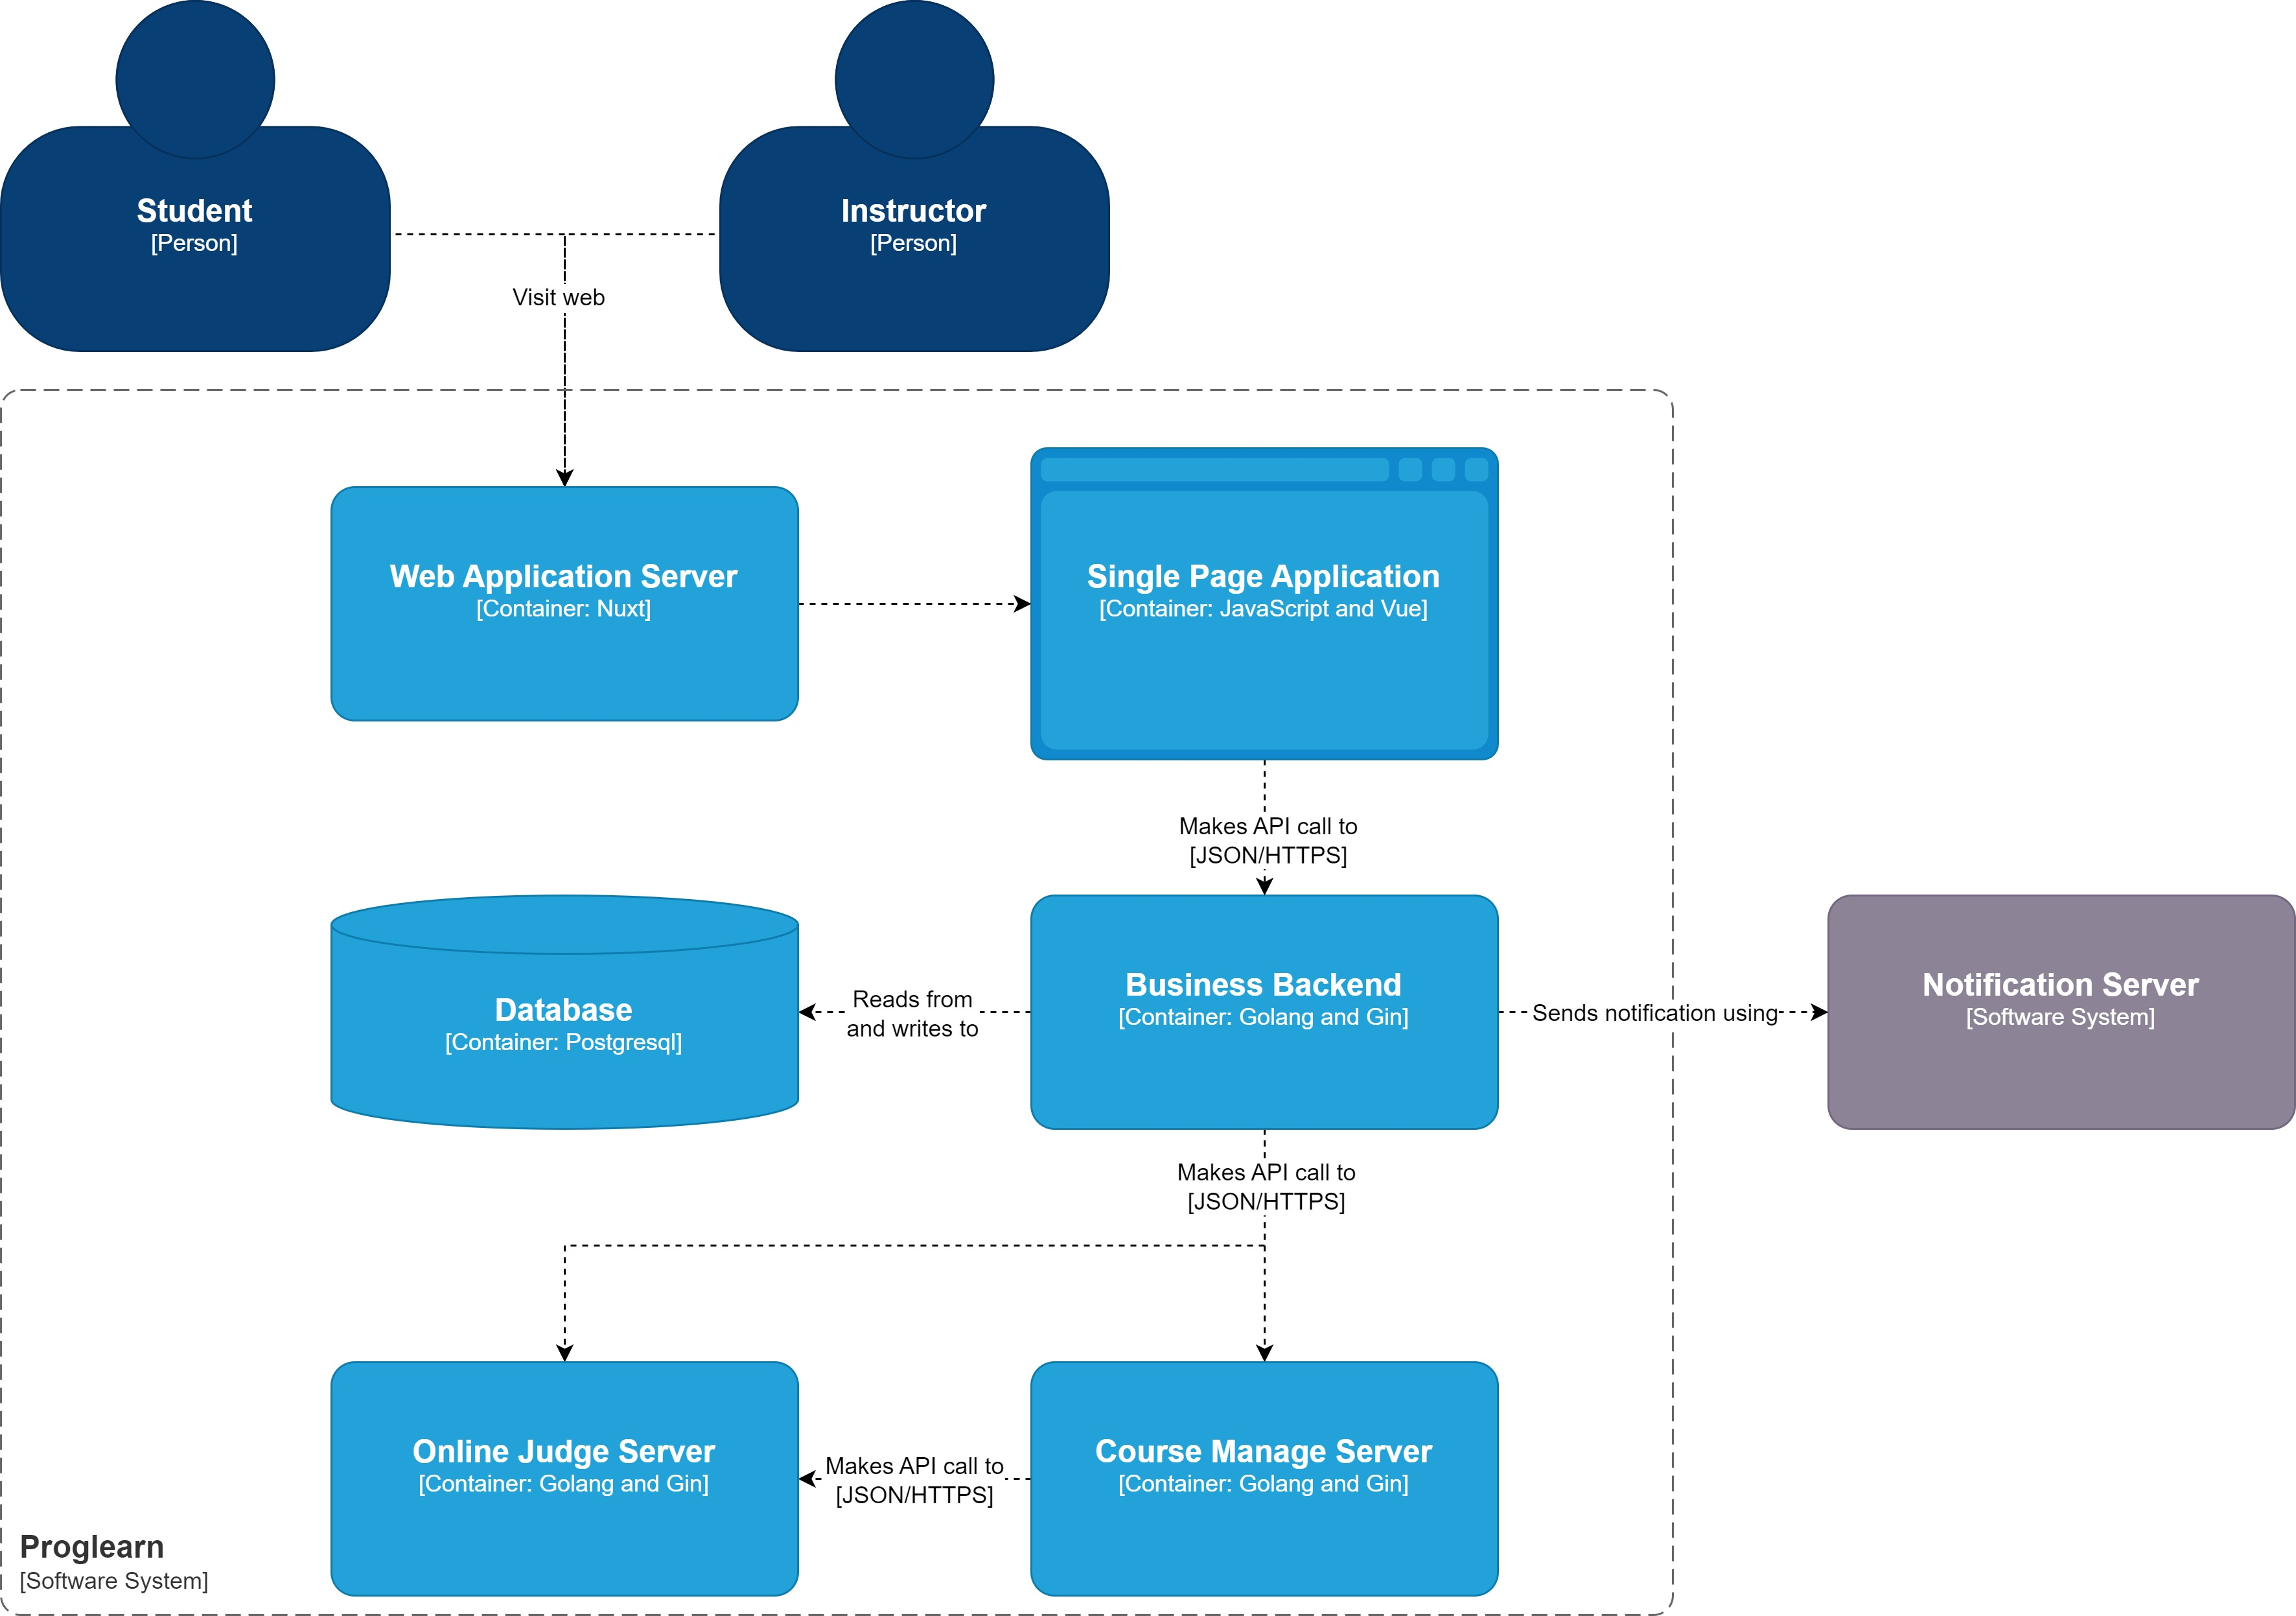
\includegraphics[width=0.7\textwidth]{./img/arc1.jpg}
          \caption{Proglearn 系統架構}
          \label{arc1}
        \end{figure}
        \begin{figure}[htbp]
          \centering
          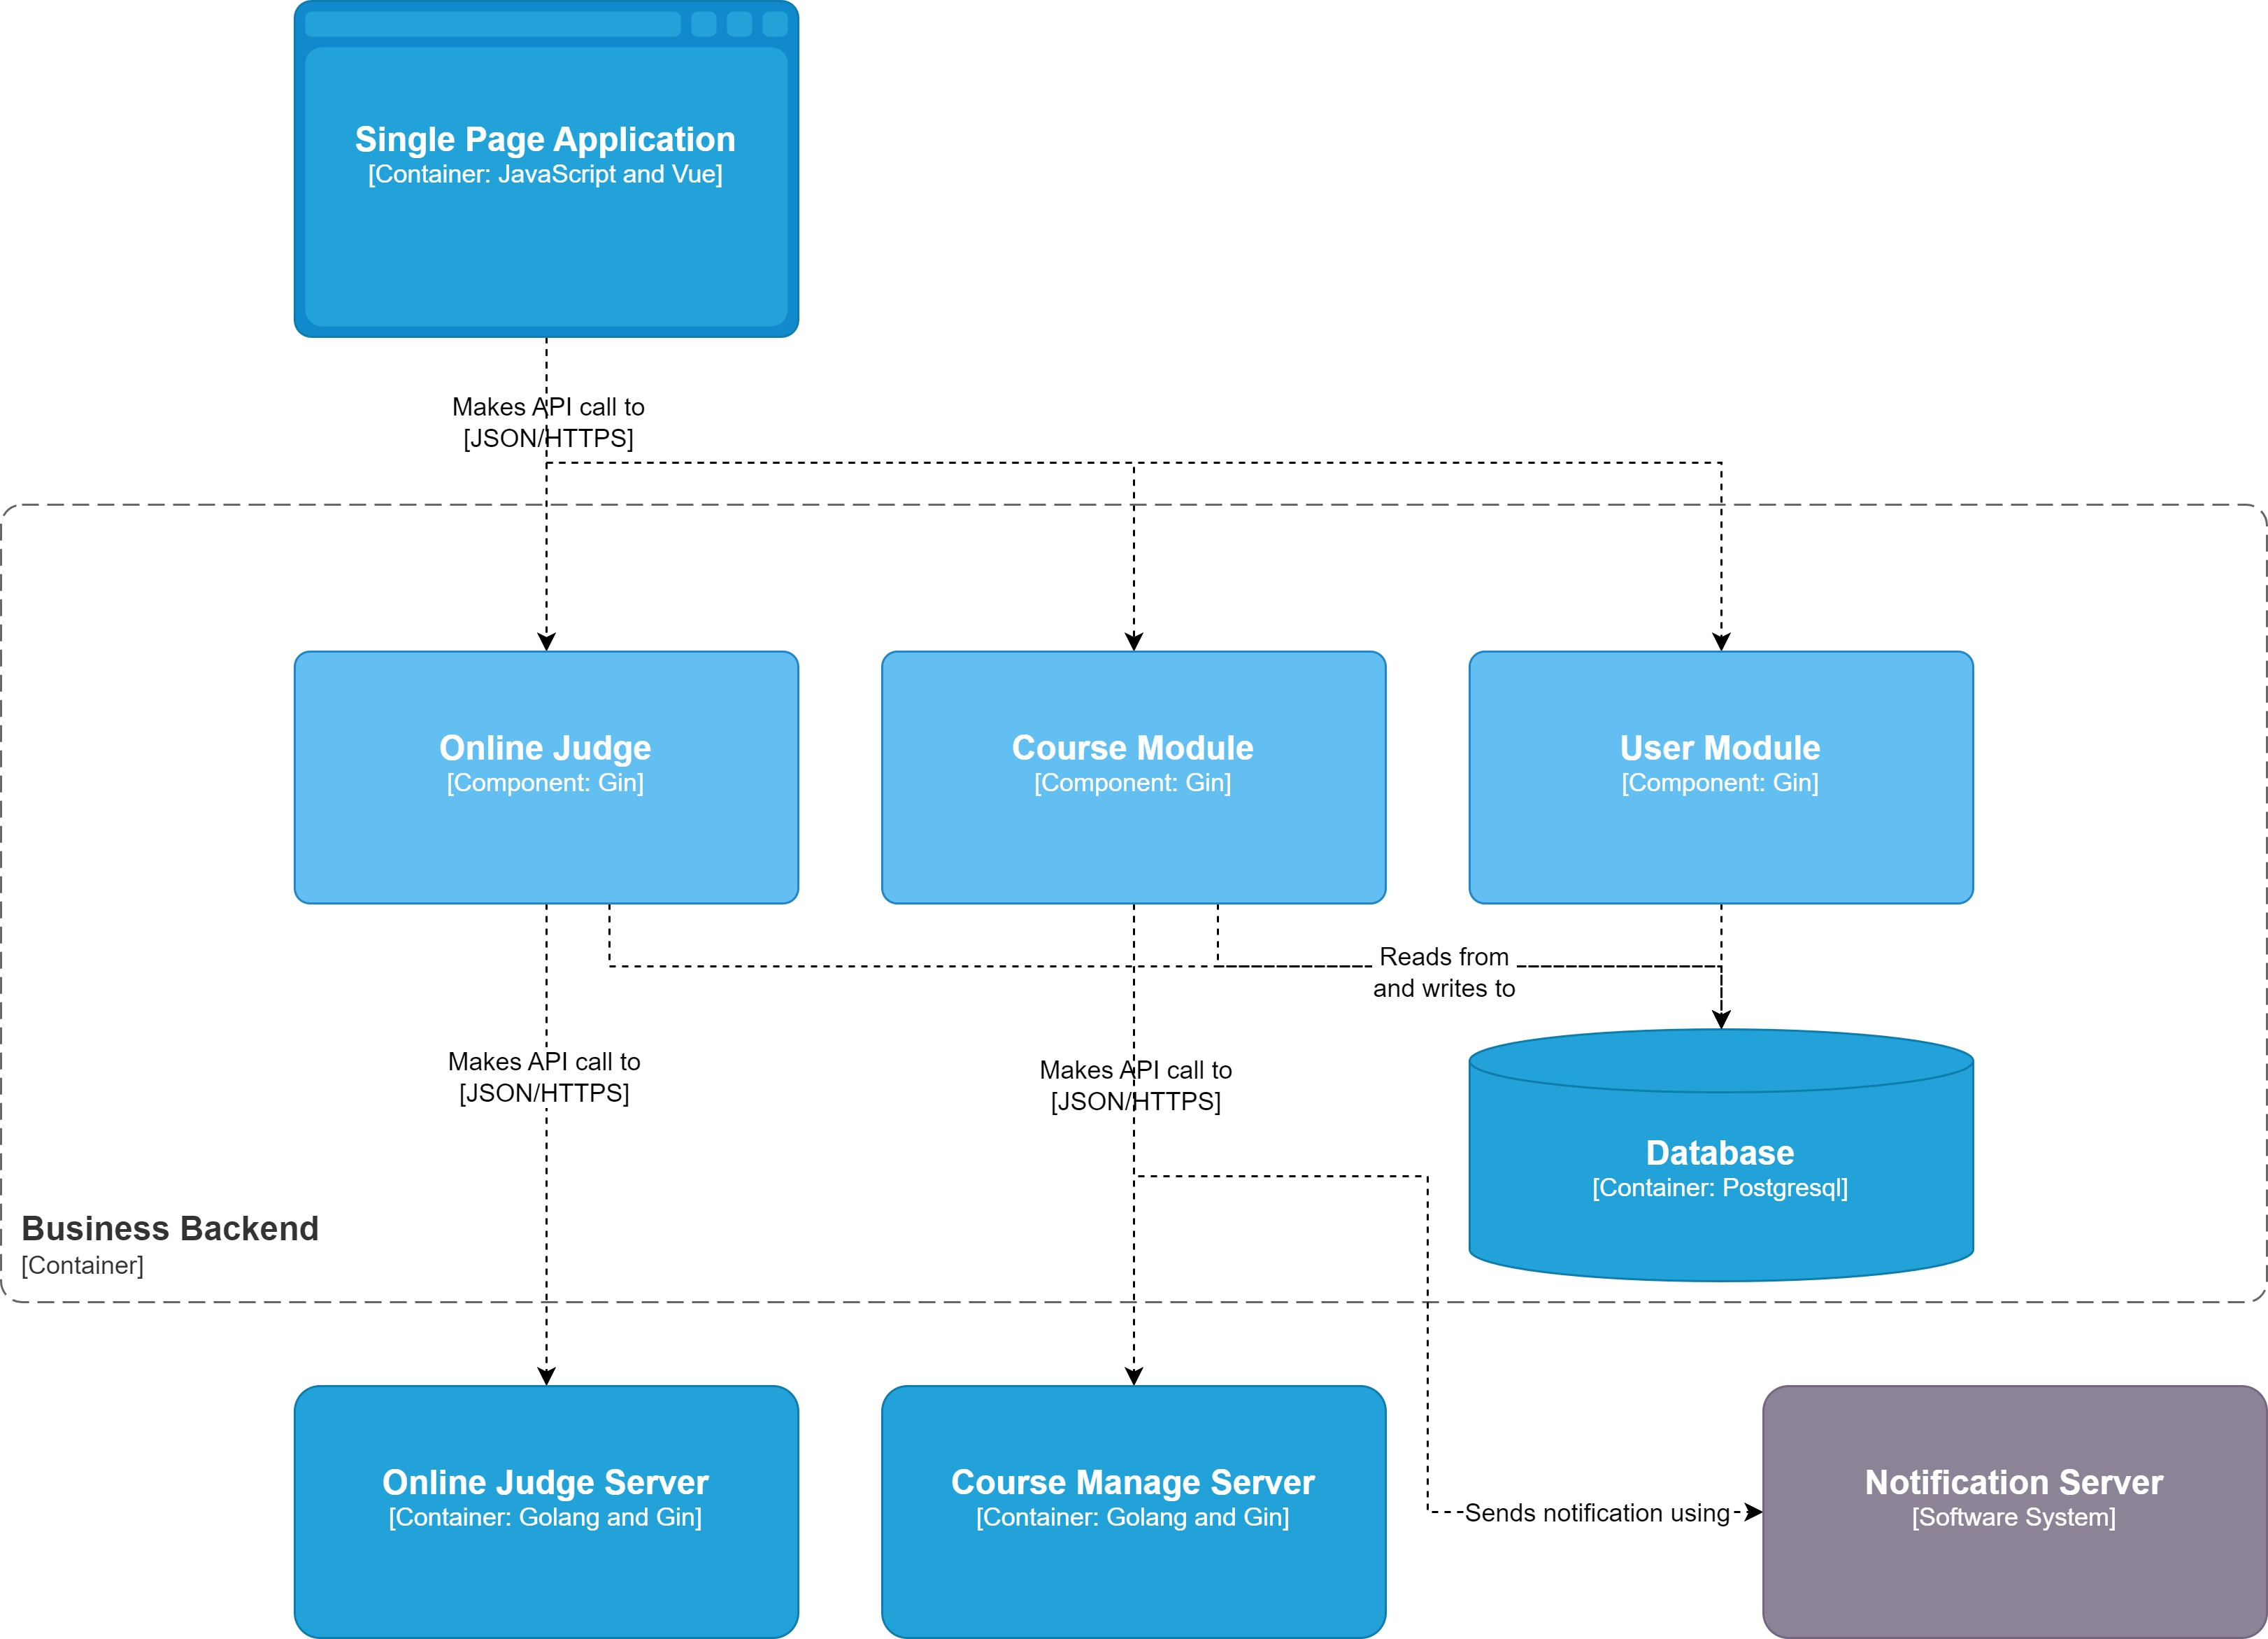
\includegraphics[width=0.65\textwidth]{./img/arc2.jpg}
          \caption{主要後端服務器架構}
          \label{arc2}
        \end{figure}
        \begin{figure}[htbp]
          \centering
          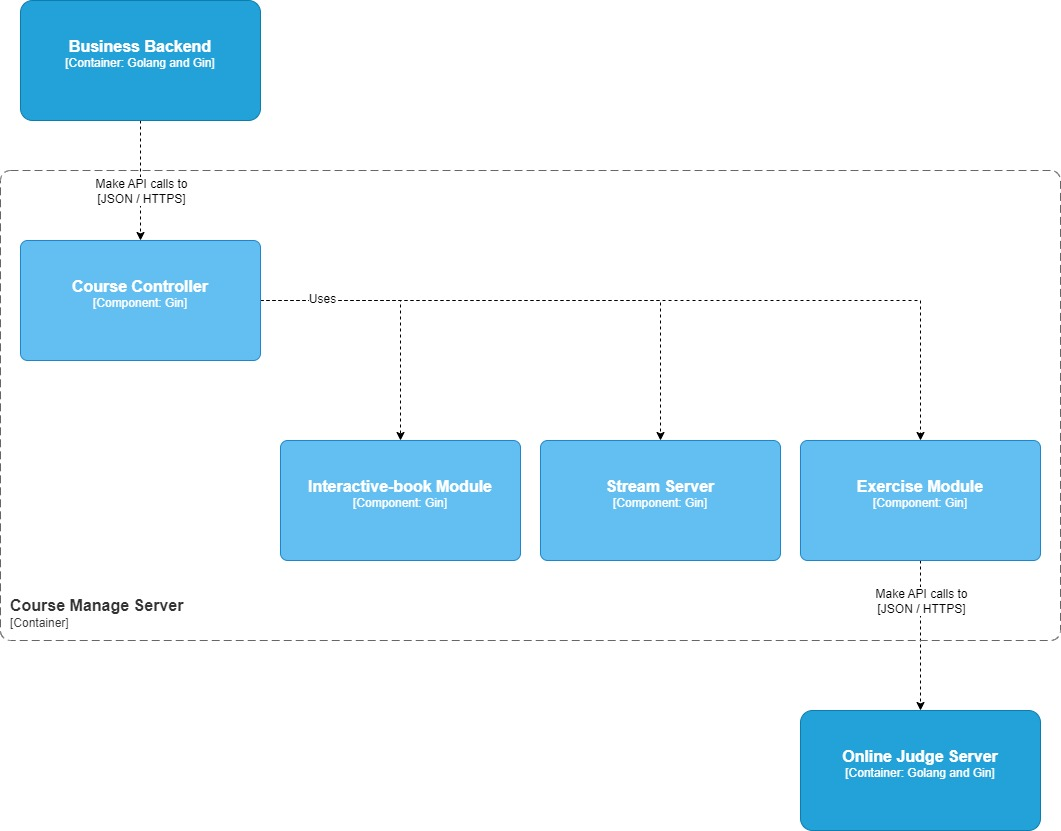
\includegraphics[width=0.7\textwidth]{./img/arc3.jpg}
          \caption{課程管理服務器架構}
          \label{arc3}
        \end{figure}
        \begin{figure}[htbp]
          \centering
          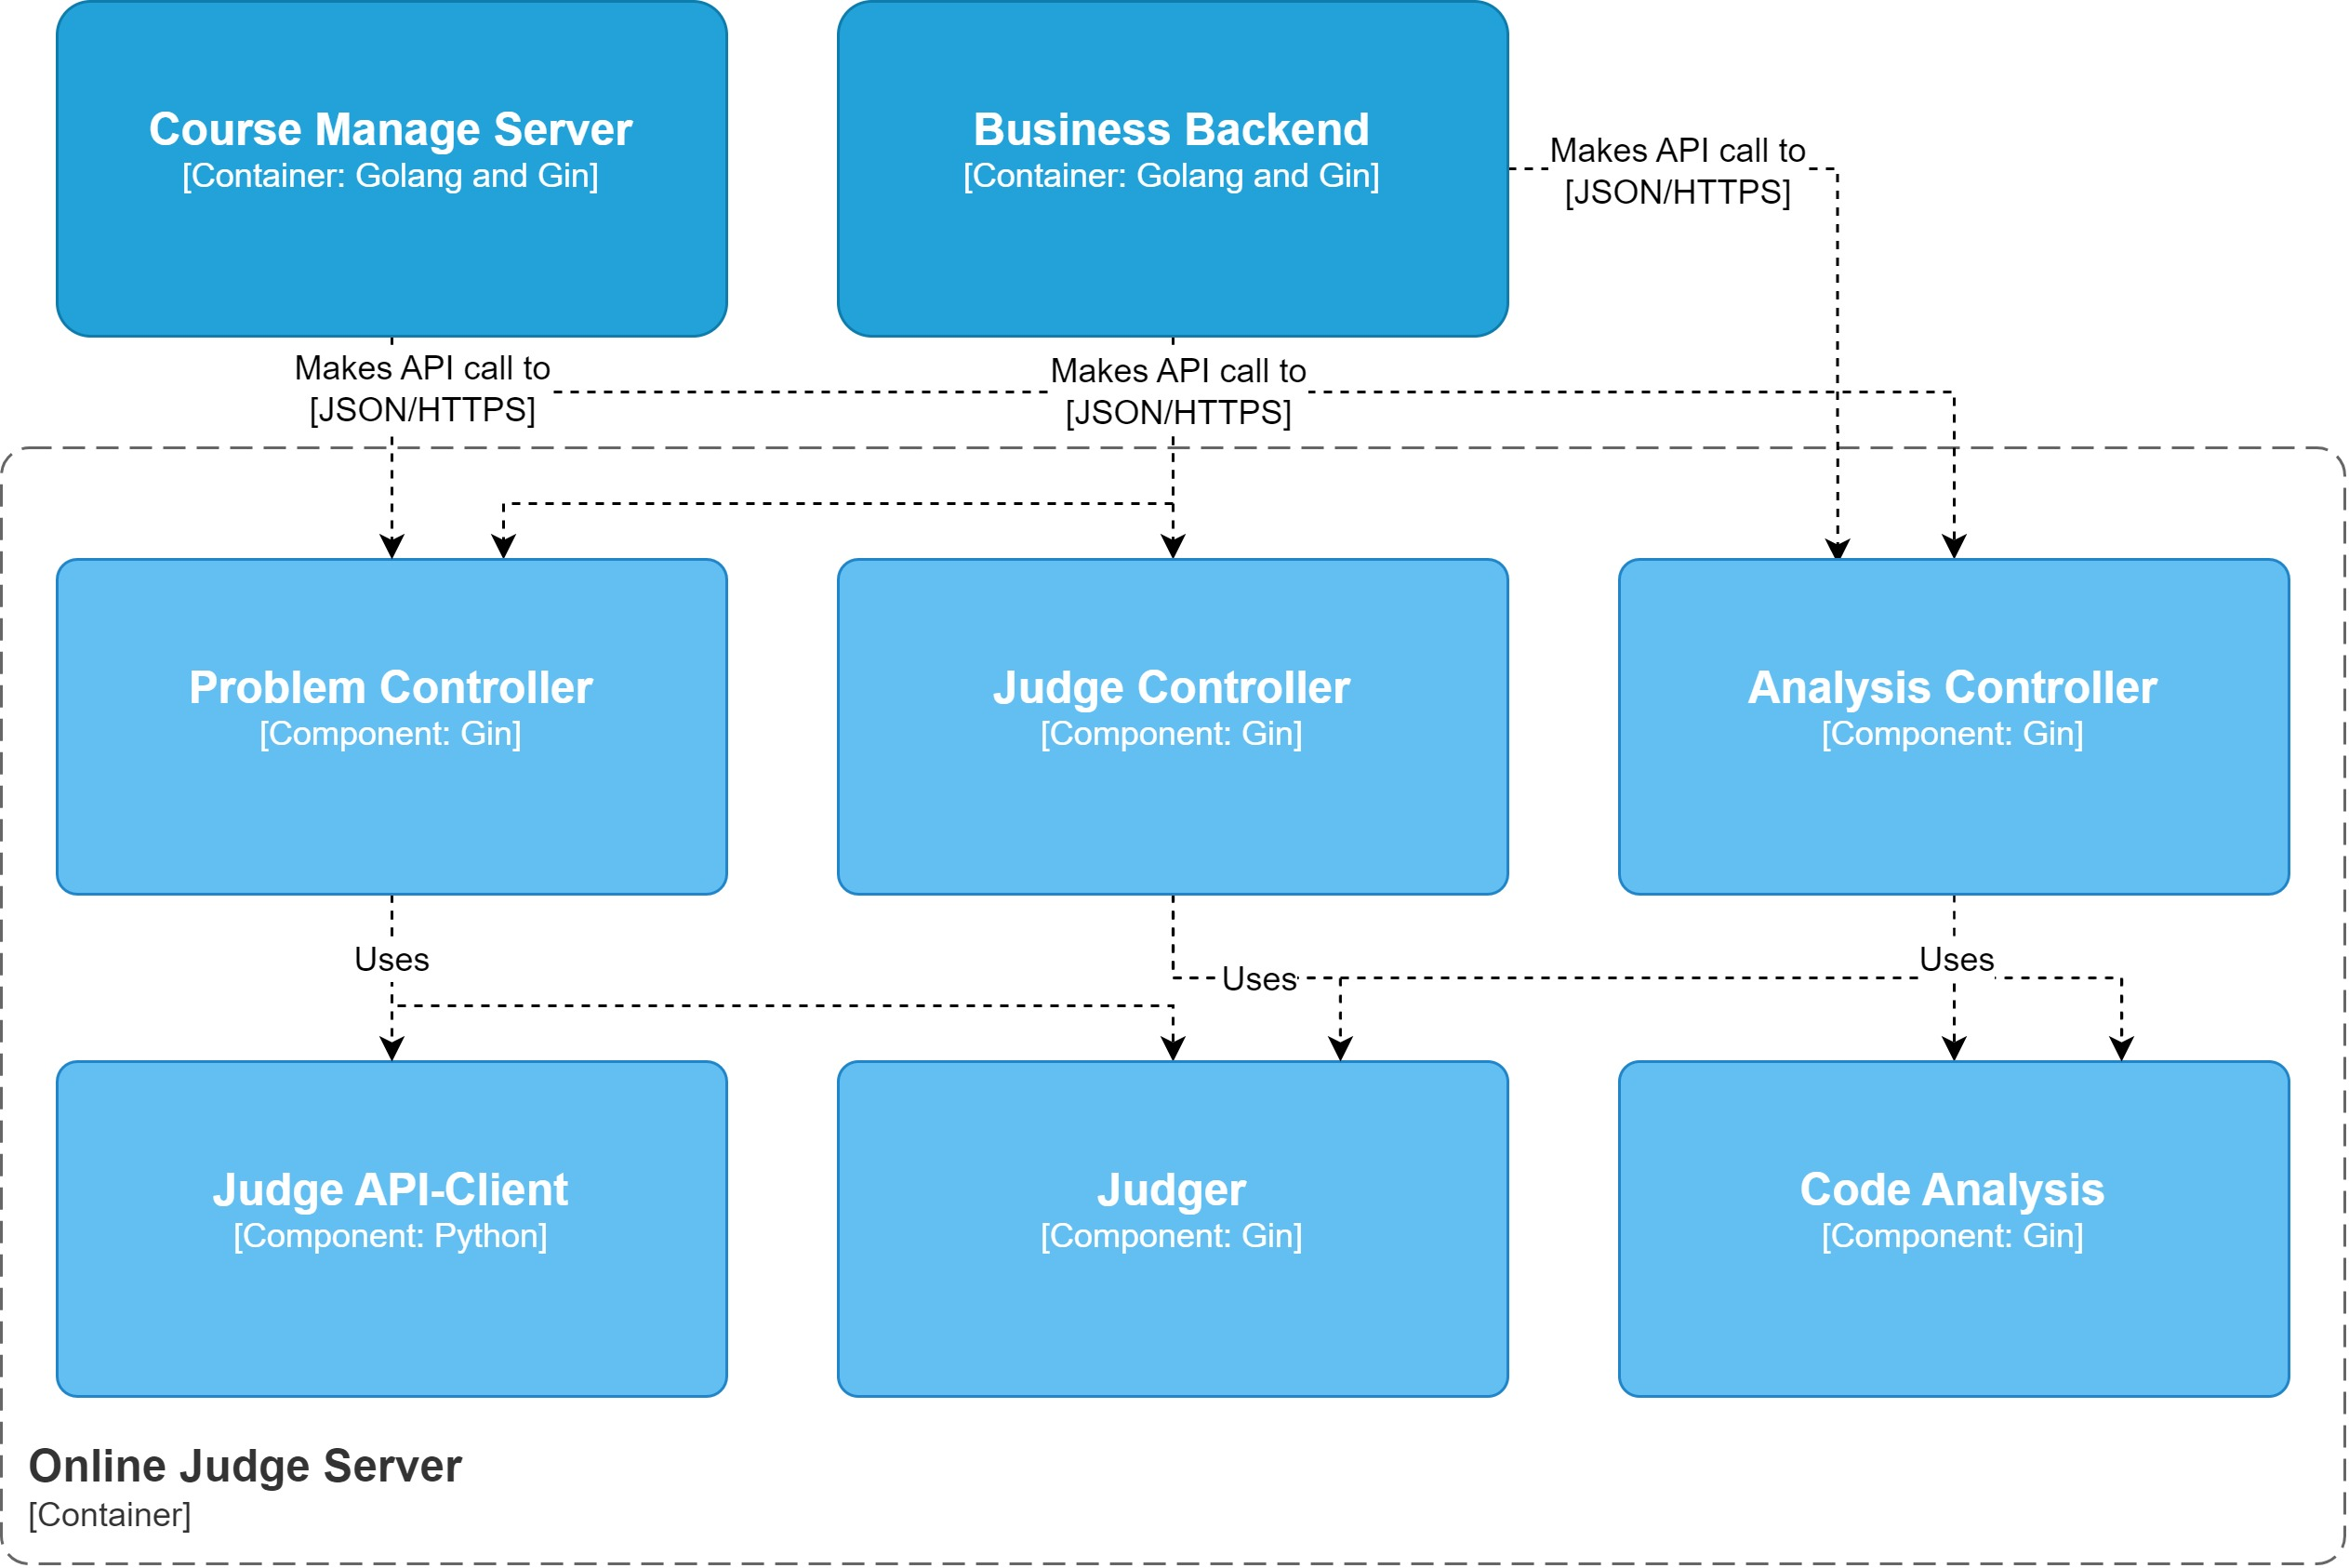
\includegraphics[width=0.7\textwidth]{./img/arc4.jpg}
          \caption{線上解題服務器架構}
          \label{arc4}
        \end{figure}
        \par 主要後端服務器(如圖\ref{arc2})
          負責處理與管理使用者資料(User Module)、課程模組(Course Module)、題目模組(Online Judge)。
        \par 課程管理服務器(如圖\ref{arc3})
          包括影片服務器(Video Server)、投影片模組(Code-Slides Module)、練習模組(Exercise Module)。
          投影片模組將使用 CodeMirror 作為編輯器,並且提供使用 JavaScript 程式碼撰寫投影片。
          % 接著使用
        \par 線上解題服務器(如圖\ref{arc4})
          包括線上題目抓取模組(Judge API-Client)、程式碼批改模組(Judger)、程式碼分析模組(Code Analysis)。
          Judge API-Client 是使用開源專案 api-client \cite{apiclient} 作為線上題目抓取模組,方便教師可以使用現有的題目做修改。
          Judger 是參考開源專案 go-judge \cite{judger1} 、JudgeServer \cite{judger2} 開發出沙盒程式碼執行環境及程式碼批改模組。
          Code Analysis 將採用多標籤辨識模型實現,後續章節將針對此核心技術進行更詳細的說明。
      \item 核心技術設計
        \begin{enumerate}
            \setlength{\parindent}{2em}
            \item Code Analysis 
            \par 程式碼分析及自動回饋是本研究的核心技術,我們將使用多標籤辨識模型來實現。
            \par 本研究規劃實驗步驟如圖\ref{ai}所示。我們採用 CodeForces 網站的題目作為訓練資料,
            CodeForces 是俄羅斯的一個程式競賽網站,提供了大量的程式競賽題目,用戶在上面作答的程式碼都會公布,
            並且還有大部分的題目都有明確的難度指標,難度指標在 800 到 3500 之間,難度指標數字越高,題目越難。
            CodeForces 有提供 API 可以取得題目的資訊,
            因此我們可以在 CodeForces 上取得題目的資訊及用戶的程式碼、輸出資料、正確答案,
            並將用戶的程式碼刪除註解、非英文字元、程式碼無法解析成抽象語法樹的資料後,再進行分析。
            我們最一開始會從難度 800 的題目作為初始訓練資料,並且人工標上錯誤類別後進行訓練模型,
            之後提升難度到 1000 的題目,先以原本的模型進行預測,再進行人工審查。            
            \begin{figure}[htbp]
              \centering
              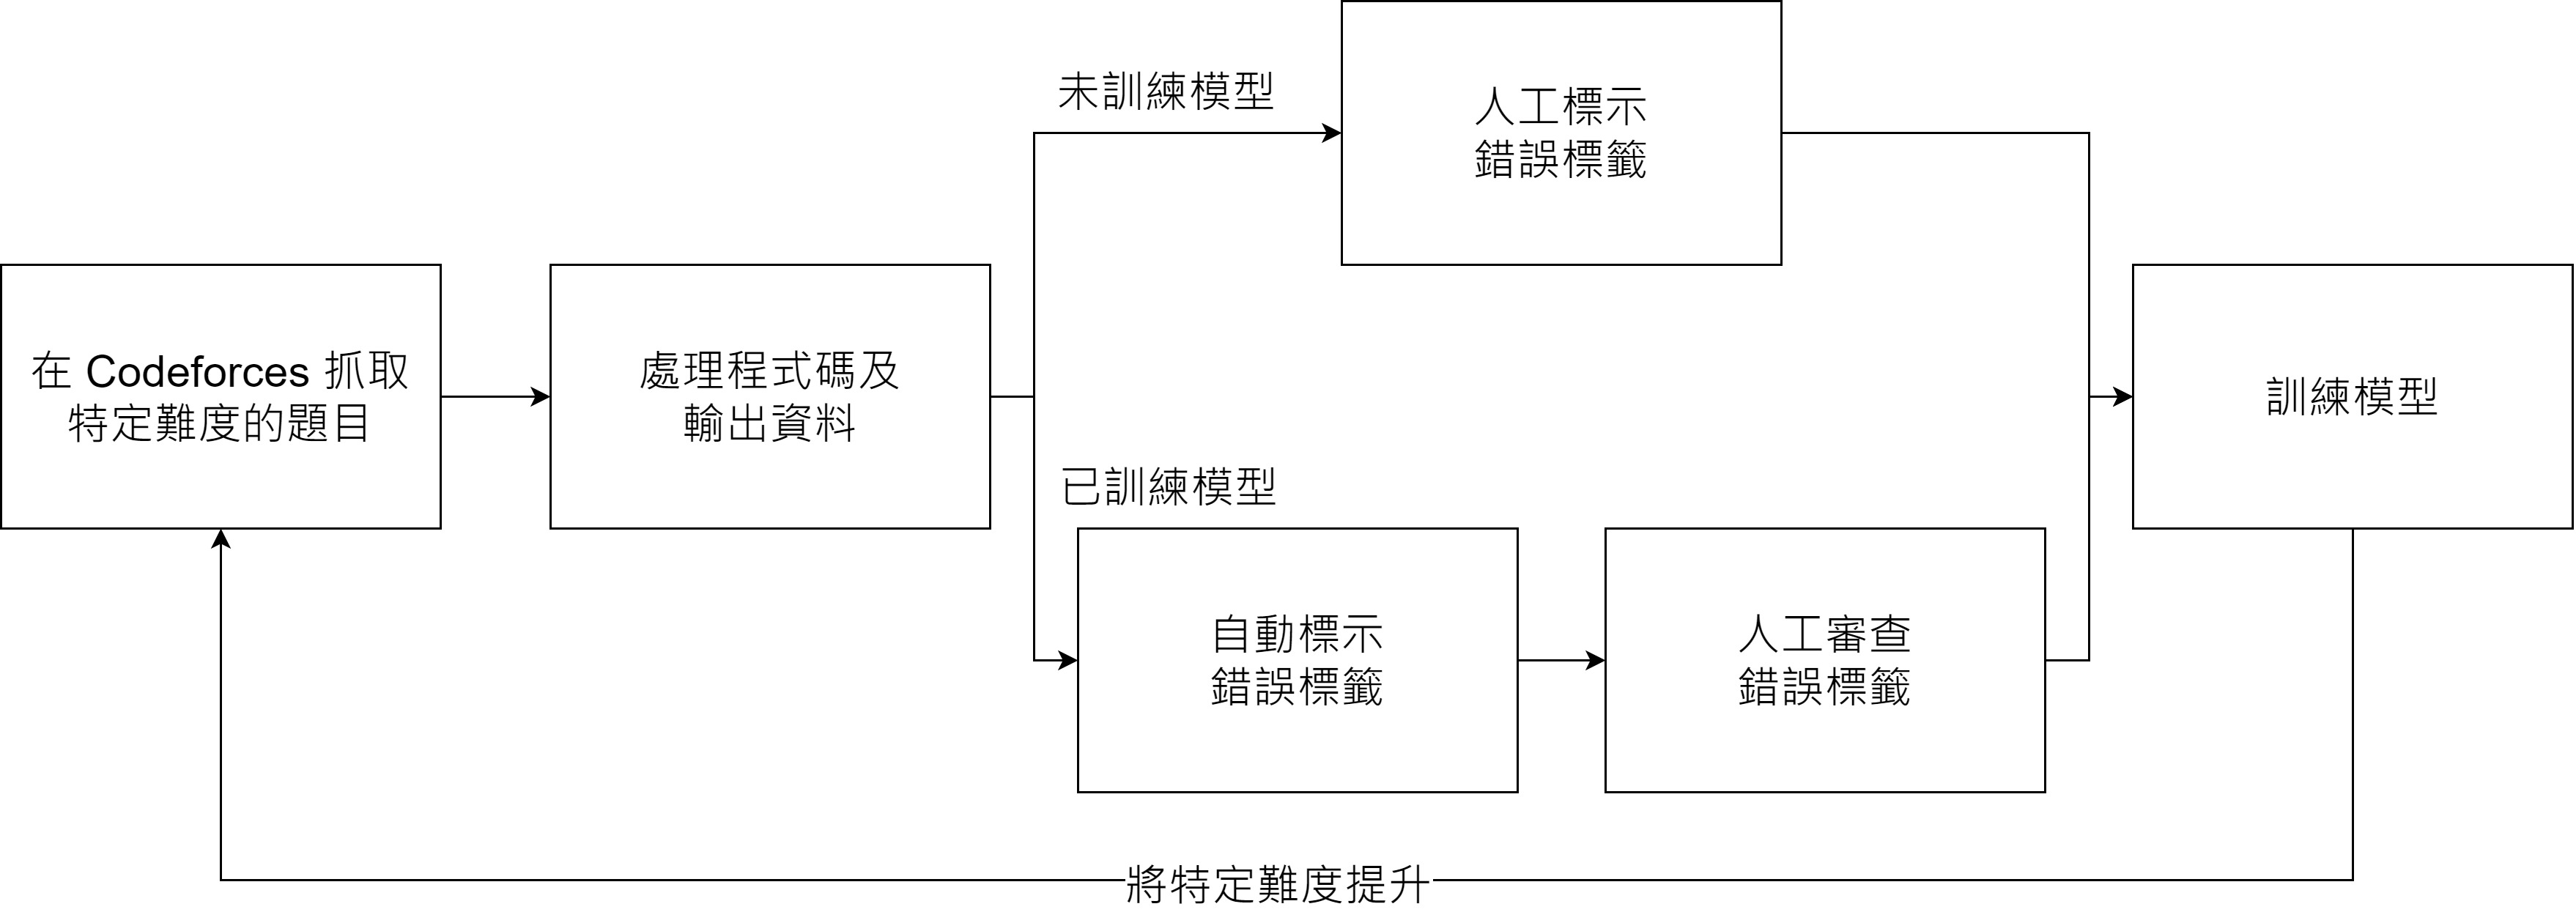
\includegraphics[width=1\textwidth]{./img/ai.jpg}
              \caption{AI}
              \label{ai}
            \end{figure}
        \end{enumerate}

    \end{enumerate}

  \item 預期結果
    \par 最後我們開發出一個整合式教學系統,
    將解決以下四個問題:
    \begin{enumerate}
      \item 教師在教學與備課的工作量大: 自動回饋系統能夠節省教師的時間。教師可以快速了解學生的學習進度和弱點,有更多的時間去創造更好的學習環境和教學資源。
      \item 受技術限制的教學方式: 透過同步練習與課後練習並輔以AI自動批改,讓教師能夠快速掌握學生的學習狀況,提高了教學效率。
      \item 師生間缺乏互動性: 互動式簡報模組,可以讓教師與學生之前有更多的互動,讓學生能夠更加主動地參與學習,並且能夠得到及時的回饋和指導。
      \item 教學工具種類繁多且功能單一: 整合式系統可以讓教師在同一個平台上創建和管理課程、學生,並能夠快速分析學生的學習狀況,提高了教學效率。
    \end{enumerate}

  \item 參考文獻
    \renewcommand{\section}[2]{}
    \begin{thebibliography}{99}  
      \bibitem{ref1} 線上解題系統:演算法競賽中,用以評測程式碼正確性的系統,可用於練習、求職面試以及競賽。
      \bibitem{ref2} 十二年國民基本教育課程綱要。民112年2月14日,取自:https://www.naer.edu.tw/PageSyllabus?fid=52。
      \bibitem{ref3} 政府資料公開平台(民111年6月29日)。全臺灣各級學校之學生數及畢業生數資料。民112年2月14日,取自:https://data.gov.tw/dataset/31436。
      \bibitem{ref4} 張瑞賓, and 李建華. "遠距教學常態化問題之探討與建議." 臺灣教育評論月刊 10.6 (2021): 27-34.
      \bibitem{ref5} 聯合新聞網(民110年3月8日)。中小學資訊教師荒! 多校找自然師兼任遭批不專業。民112年2月14日,取自:https://udn.com/news/story/6885/5303319。
      \bibitem{ref6} 資訊教室的廣播與管理系統:針對資訊教室的廣播與管理系統,可將電腦畫面傳送給特定或所有用戶端,並且能監控用戶端的電腦畫面。
      \bibitem{ref7} 岳修平. "即時群播遠距教學之班級經營." (2000): 63-74.
      \bibitem{ref8} De Giusti, Armando. "Book review: Policy brief: Education during COVID-19 and beyond." Revista Iberoamericana de Tecnología En Educación y Educación En Tecnología 26 (2020): 110-111.
      \bibitem{ref9} Tumwesige, Josephine. "COVID-19 Educational disruption and response: Rethinking e-Learning in Uganda." University of Cambridge (2020).
      \bibitem{ref10} Santos, Joseline M., and Rowell DR Castro. "Technological Pedagogical content knowledge (TPACK) in action: Application of learning in the classroom by pre-service teachers (PST)." Social Sciences \& Humanities Open 3.1 (2021): 100110.
      \bibitem{ref11} Ratheeswari, K. "Information communication technology in education." Journal of Applied and Advanced research 3.1 (2018): 45-47.
      \bibitem{ref12} Forbes 2000
      \bibitem{ref13} Ouya, Samuel, et al. "WebRTC platform proposition as a support to the educational system of universities in a limited Internet connection context." 2015 5th World Congress on Information and Communication Technologies (WICT). IEEE, 2015.
      \bibitem{ref14} Ibrahim, Mohamed, and Osama Al-Shara. "Impact of interactive learning on knowledge retention." Lecture Notes in Computer Science 4558 (2007): 347.
      \bibitem{ref15} Akram, Huma, et al. "Technology integration in higher education during COVID-19: An assessment of online teaching competencies through technological pedagogical content knowledge model." Frontiers in psychology 12 (2021): 736522.
      \bibitem{ref16} Krusche, Stephan, and Andreas Seitz. "Artemis: An automatic assessment management system for interactive learning." Proceedings of the 49th ACM technical symposium on computer science education. 2018.
      \bibitem{ref17} Dong, Yu, Jingyang Hou, and Xuesong Lu. "An intelligent online judge system for programming training." Database Systems for Advanced Applications: 25th International Conference, DASFAA 2020, Jeju, South Korea, September 24–27, 2020, Proceedings, Part III 25. Springer International Publishing, 2020.
      \bibitem{apiclient} api-client. Available from: https://github.com/online-judge-tools/api-client
      \bibitem{judger1} go-judge. Available from: https://github.com/criyle/go-judge
      \bibitem{judger2} JudgeServer. Available from: https://github.com/helsonxiao/JudgeServer
    \end{thebibliography} 

  \item 需要指導教授內容
    \begin{enumerate}
      \setlength{\parindent}{2em}
      \item 資料收集:學習資料與文獻收集、分析與整理之方法。
      \item 技術分析:學習分析各個功能可能會使用到的相關技術。
      \item 研究方法及步驟:學習利用物件導向軟體工程技術、機器學習技術、
      Web技術來規劃軟體之架構與細部設計。
      \item 系統測試與部署:學習設計不同的測試案例及運用不同的測試方法,以確保本系統之可用性與可靠度,
      並學習如何運用持續整合/部署以及容器技術,進行系統自動化建置與發佈。
    \end{enumerate}
\end{enumerate}
\end{document}